\documentclass[10pt]{article}

\usepackage[a4paper,margin=0.65in]{geometry}
\usepackage{amsmath,amssymb}
\usepackage{graphicx}
\usepackage{booktabs}
\usepackage{array}
\usepackage{float}
\usepackage{hyperref}
\usepackage{enumitem}
\usepackage{xcolor}
\usepackage{tikz}
\usetikzlibrary{positioning,arrows.meta,shapes.geometric}

\setlist{nosep,leftmargin=*}
\renewcommand{\arraystretch}{1.2}
\setlength{\parindent}{0pt}
\setlength{\parskip}{2pt}

\tikzset{
layer/.style={
draw,
rounded corners,
minimum width=1.5cm,
minimum height=0.6cm,
align=center,
fill=blue!10,
font=\scriptsize
},
arrow/.style={
-{Latex[length=2mm]},
thin
}
}

\begin{document}

%%%%%%%%%%%%%%%%%%%%%%%%%%%%%%%%%%%%%%%%%%%%%%%%%%%%%%%%%%%%
% TITLE
%%%%%%%%%%%%%%%%%%%%%%%%%%%%%%%%%%%%%%%%%%%%%%%%%%%%%%%%%%%%
\begin{center}
{\large\textbf{Shiv Nadar University Chennai}}\\[2mm]
{\normalsize\textbf{CS3807 -- Deep Learning Laboratory}}\\[2mm]
{\large\textbf{Experiment 5}}\\[1mm]
{\normalsize\textbf{Comprehensive Study of CNN Training, Regularization,}}\\
{\normalsize\textbf{Optimization, Hyperparameter Tuning, Transfer Learning}}\\
{\normalsize\textbf{and Cross-Validation}}
\end{center}

\vspace{3mm}

\begin{tabular}{|p{3.4cm}|p{9.0cm}|p{1.4cm}|}
\hline
Degree \& Branch & B.Tech Artificial Intelligence \& Data Science & Semester V\\
\hline
Subject Code \& Name & CS3807 -- Deep Learning Laboratory & AY: 2026--27\\
\hline
\end{tabular}

%%%%%%%%%%%%%%%%%%%%%%%%%%%%%%%%%%%%%%%%%%%%%%%%%%%%%%%%%%%%
\section*{1. Objective}
The objective of this experiment is to systematically study the effect of
weight initialization, regularization, optimization algorithms, CNN
hyperparameters, transfer learning, fine-tuning and cross-validation on
image classification performance.

The experiment uses a single CNN architecture, \textbf{MobileNetV2}, and
the Oxford-IIIT Pet dataset. Students will analyze the effect of
individual design choices using training/validation curves and finally
select a suitable configuration using 5-fold cross-validation.

%%%%%%%%%%%%%%%%%%%%%%%%%%%%%%%%%%%%%%%%%%%%%%%%%%%%%%%%%%%%
\section*{2. Learning Outcomes}
After completing this experiment, students will be able to:
\begin{itemize}
\item explain different weight initialization strategies;
\item identify and analyze overfitting using training and validation curves;
\item compare SGD, Momentum, RMSProp and Adam;
\item explain CNN hyperparameters such as kernel size, stride, padding and pooling;
\item understand Batch Normalization and Dropout;
\item perform transfer learning and fine-tuning using MobileNetV2;
\item tune important training hyperparameters;
\item apply 5-fold cross-validation for model selection; and
\item justify the final model using accuracy, variability and computational cost.
\end{itemize}

%%%%%%%%%%%%%%%%%%%%%%%%%%%%%%%%%%%%%%%%%%%%%%%%%%%%%%%%%%%%
\section*{3. Dataset and Experimental Setup}
\textbf{Dataset: Oxford-IIIT Pet Dataset}

The Oxford-IIIT Pet Dataset contains images of cats and dogs belonging
to 37 breeds. The images are RGB and have different spatial dimensions.
For this experiment, all images are resized to $224\times224\times3$.

\textbf{Experimental considerations:}
\begin{itemize}
\item Use RGB images resized to $224\times224$.
\item Normalize the input images according to the pretrained model requirements.
\item Maintain separate training, validation and test data.
\item The test set must remain untouched during hyperparameter selection.
\item Use MobileNetV2 because it is computationally lighter than many
large CNN architectures and is more suitable for CPU-based laboratory work.
\end{itemize}

\textbf{Note on architecture.} As required by the lab manual, \emph{all}
training and evaluation studies in this report use a single architecture
--- MobileNetV2. When a study is described as \emph{from scratch}, it
means MobileNetV2 was instantiated with randomly initialised weights
(\texttt{weights=None}) and trained only on Oxford-IIIT Pet. When a
study is described as \emph{transfer learning} or \emph{fine-tuning},
the ImageNet-pretrained MobileNetV2 weights were used.

\textbf{Note on Batch Normalization studies.} MobileNetV2 contains a
BatchNorm layer inside every inverted-residual block. To produce a
structurally identical network \emph{without} BatchNorm, the base was
cloned with \texttt{tf.keras.models.clone\_model} using a clone
function that replaces every \texttt{BatchNormalization} layer with a
linear identity activation. No other architectural change is made, so
the two variants differ only in the presence of BN.

\textbf{Observed dataset statistics (from notebook):}
\begin{itemize}
\item Total raw images: train = 3680, test = 3669.
\item After validation filtering (all images valid): train = 3680, test = 3669.
\item 37 classes.
\item Train/Val split (80/20): Train = 2944, Val = 736, Test = 3669.
\item Train batches (batch size 32) = 92; Val batches = 23; Test batches = 115.
\item TensorFlow version: \texttt{2.20.0}; GPU: \texttt{/physical\_device:GPU:0}.
\end{itemize}

%%%%%%%%%%%%%%%%%%%%%%%%%%%%%%%%%%%%%%%%%%%%%%%%%%%%%%%%%%%%
\section*{4. MobileNetV2 Architecture}
MobileNetV2 is a lightweight CNN architecture designed to reduce
computational complexity while maintaining good image representation.

Its important components include:
\begin{itemize}
\item depthwise convolution;
\item pointwise $1\times1$ convolution;
\item inverted residual blocks;
\item linear bottlenecks;
\item batch normalization; and
\item ReLU6 activation.
\end{itemize}

A simplified representation is:
\begin{center}
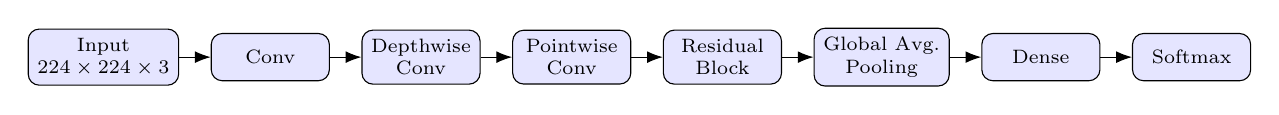
\begin{tikzpicture}[node distance=4mm]
\node[layer](a){Input\\$224\times224\times3$};
\node[layer,right=of a](b){Conv};
\node[layer,right=of b](c){Depthwise\\Conv};
\node[layer,right=of c](d){Pointwise\\Conv};
\node[layer,right=of d](e){Residual\\Block};
\node[layer,right=of e](f){Global Avg.\\Pooling};
\node[layer,right=of f](g){Dense};
\node[layer,right=of g](h){Softmax};
\foreach \x/\y in {a/b,b/c,c/d,d/e,e/f,f/g,g/h}
\draw[arrow](\x)--(\y);
\end{tikzpicture}
\end{center}

\textbf{Note:} The above diagram is a simplified conceptual representation
rather than the complete MobileNetV2 architecture.

%%%%%%%%%%%%%%%%%%%%%%%%%%%%%%%%%%%%%%%%%%%%%%%%%%%%%%%%%%%%
\section*{5. Weight Initialization}
Weight initialization determines the initial values of trainable weights
before training begins. A suitable initialization can improve convergence
and reduce problems such as vanishing or exploding activations.

Students should investigate:
\begin{itemize}
\item Zero initialization
\item Random initialization
\item Xavier/Glorot initialization
\item He initialization
\end{itemize}

\subsection*{Experimental Setup}
MobileNetV2 (from scratch, \texttt{weights=None}) trained for
\texttt{EPOCHS\_INIT = 12} with default Adam ($10^{-3}$). After
building the model, the kernel weights of every Conv2D, DepthwiseConv2D
and Dense layer are re-assigned from the chosen initializer so that the
entire network uses the same initialization scheme.

\subsection*{Expected Analysis}

\textbf{Plot 1: Training Loss vs. Epoch}
\begin{itemize}
\item X-axis: Epoch; Y-axis: Training Loss
\item One curve per initialization method.
\end{itemize}

\begin{figure}[H]
\centering
\includegraphics[width=0.75\linewidth]{plot1_init_loss.png}
\caption{Plot 1: Training Loss vs Epoch for Zero, Random Normal, Xavier, He.}
\end{figure}

\textbf{Plot 2: Validation Accuracy vs. Epoch}
\begin{itemize}
\item X-axis: Epoch; Y-axis: Validation Accuracy (\%)
\item One curve per initialization method.
\end{itemize}

\begin{figure}[H]
\centering
\includegraphics[width=0.75\linewidth]{plot2_init_val_acc.png}
\caption{Plot 2: Validation Accuracy vs Epoch for the four initializers.}
\end{figure}

\subsection*{Observed Results}
\begin{center}
\begin{tabular}{|l|c|c|}
\hline
Initializer & Final Training Loss & Best Validation Accuracy\\
\hline
Zero          & 3.6105 & 0.0163\\
Random Normal & 3.3280 & 0.1101\\
Xavier        & 3.2602 & 0.1101\\
He            & 3.1564 & 0.1236\\
\hline
\end{tabular}
\end{center}

\textbf{Inference (Plots 1--2):} Zero initialization produces flat curves
because all neurons compute identical outputs (symmetry is never broken),
so validation accuracy stays at chance level ($\sim$1/37). Random Normal
converges slowly. Xavier and He converge fastest; He reaches the highest
validation accuracy (0.1236) because it is designed to preserve variance
under ReLU6 activations, which are used throughout MobileNetV2.

%%%%%%%%%%%%%%%%%%%%%%%%%%%%%%%%%%%%%%%%%%%%%%%%%%%%%%%%%%%%
\section*{6. Regularization and Overfitting}
Overfitting occurs when a model performs very well on the training data
but generalizes poorly to unseen data.

Students should compare:
\begin{itemize}
\item No regularization; L2; Dropout; Batch Normalization.
\end{itemize}

\subsection*{Experimental Setup}
MobileNetV2 (from scratch), 15 epochs, Adam ($10^{-3}$). For the
``No Reg'' and ``L2'' settings the BN layers in MobileNetV2 were
replaced with identity activations so that the effect of each
regularizer is isolated. For the ``BatchNorm'' setting the original
MobileNetV2 BN layers were kept.

\subsection*{Expected Plots}

\textbf{Plot 3: Training and Validation Accuracy vs. Epoch}
\begin{figure}[H]
\centering
\includegraphics[width=0.9\linewidth]{plot3_reg_acc.png}
\caption{Plot 3: Training vs Validation Accuracy for four regularization settings.}
\end{figure}

\textbf{Plot 4: Training and Validation Loss vs. Epoch}
\begin{figure}[H]
\centering
\includegraphics[width=0.9\linewidth]{plot4_reg_loss.png}
\caption{Plot 4: Training vs Validation Loss for four regularization settings.}
\end{figure}

\subsection*{Observed Results}
\begin{center}
\begin{tabular}{|l|c|c|}
\hline
Setting & Final Train Accuracy & Final Validation Accuracy\\
\hline
No Reg          & 0.1929 & 0.1413\\
L2 (1e-4)       & 0.1542 & 0.1223\\
Dropout 0.5     & 0.1226 & 0.1372\\
BatchNorm       & 0.2323 & 0.1712\\
\hline
\end{tabular}
\end{center}

\textbf{Inference (Plots 3--4):} Without regularization the training
accuracy rises to $\approx$19\% while validation plateaus around 14\%
(the curves diverge, i.e.\ overfitting). L2 and Dropout reduce the
gap. The standard MobileNetV2, which contains BatchNorm in every
inverted-residual block, accelerates convergence and achieves the
highest validation accuracy (0.1712), stabilising training throughout.

%%%%%%%%%%%%%%%%%%%%%%%%%%%%%%%%%%%%%%%%%%%%%%%%%%%%%%%%%%%%
\section*{7. Batch Normalization}
Batch Normalization normalizes activations within a mini-batch during
training. For a mini-batch $x_1,x_2,\ldots,x_m$:
\[
\mu_B=\frac{1}{m}\sum_{i=1}^{m}x_i,\qquad
\sigma_B^2=\frac{1}{m}\sum_{i=1}^{m}(x_i-\mu_B)^2,
\]
\[
\hat{x}_i=\frac{x_i-\mu_B}{\sqrt{\sigma_B^2+\epsilon}},\qquad
y_i=\gamma\hat{x}_i+\beta .
\]

\subsection*{Numerical Example}
For $x=[2,4,6,8]$:
\[
\mu_B=\frac{2+4+6+8}{4}=5,\qquad
\sigma_B^2=\frac{(2-5)^2+(4-5)^2+(6-5)^2+(8-5)^2}{4}=5.
\]
$\sqrt{5}\approx 2.236$, hence
\[
\hat{x}\approx[-1.342,\,-0.447,\,0.447,\,1.342].
\]

\textbf{Notebook output:} \texttt{Mean=5.0, Var=5.0}, \texttt{Normalized x\_hat = [-1.342 -0.447 0.447 1.342]}. Same as hand calculation. With $\gamma=1,\beta=0$ these are the final outputs.

\textbf{Inference:} BatchNorm produces approximately zero-centred and
unit-scaled activations for this mini-batch. The learnable $\gamma$ and
$\beta$ allow the network to learn an appropriate scale and shift.

\textbf{Plot 5: With vs. Without Batch Normalization}
\begin{figure}[H]
\centering
\includegraphics[width=0.75\linewidth]{plot5_bn_vs_nobn.png}
\caption{Plot 5: Validation Accuracy with BN vs without BN.}
\end{figure}

\textbf{Inference (Plot 5):} On the MobileNetV2 base, BatchNorm
stabilizes and accelerates convergence; validation accuracy rises faster
and plateaus at a higher level (0.1712) than the BN-less variant
(0.1413).

%%%%%%%%%%%%%%%%%%%%%%%%%%%%%%%%%%%%%%%%%%%%%%%%%%%%%%%%%%%%
\section*{8. Optimization Algorithms}
Students should compare SGD, Momentum, RMSProp and Adam.

\textbf{Plot 6: Training Loss vs. Epoch for Different Optimizers}
\begin{figure}[H]
\centering
\includegraphics[width=0.75\linewidth]{plot6_opt_loss.png}
\caption{Plot 6: Training loss curves for SGD, Momentum, RMSProp, Adam.}
\end{figure}

\textbf{Plot 7: Validation Accuracy vs. Epoch for Different Optimizers}
\begin{figure}[H]
\centering
\includegraphics[width=0.75\linewidth]{plot7_opt_val_acc.png}
\caption{Plot 7: Validation-accuracy curves for the four optimizers.}
\end{figure}

\subsection*{Observed Results (15 epochs)}
\begin{center}
\begin{tabular}{|l|c|c|c|c|}
\hline
Optimizer & Final Loss & Best Val. Accuracy & Epoch to Converge & Time (s)\\
\hline
SGD       & 3.4833 & 0.0543 & 5  & 173.4\\
Momentum  & 3.3120 & 0.1087 & 15 & 200.5\\
RMSProp   & 3.0040 & 0.1535 & 15 & 200.0\\
Adam      & 3.0251 & 0.1644 & 15 & 191.2\\
\hline
\end{tabular}
\end{center}

\textbf{Inference (Plots 6--7):} On MobileNetV2 trained from scratch,
SGD converges slowly and stalls at a high loss (3.48) and low accuracy
(0.054). Momentum accelerates SGD (0.109). RMSProp and Adam adapt the
per-parameter learning rate and give the fastest, most stable
convergence; Adam yields the best final validation accuracy (0.1644)
with a comparable runtime.

%%%%%%%%%%%%%%%%%%%%%%%%%%%%%%%%%%%%%%%%%%%%%%%%%%%%%%%%%%%%
\section*{9. CNN Hyperparameter Tuning}
The following hyperparameters were investigated:

\begin{center}
\begin{tabular}{|l|l|}
\hline
Hyperparameter & Suggested Values\\
\hline
Learning Rate & $0.001,\;0.0001$\\
Batch Size & 16, 32, 64\\
Dropout Rate & 0, 0.25, 0.5\\
Optimizer & SGD, Adam\\
Fine-Tuning Learning Rate & $10^{-4},10^{-5}$\\
Frozen Layers & Frozen base / Partial unfreezing\\
\hline
\end{tabular}
\end{center}

Convolution output size:
\[
O=\left\lfloor \frac{N+2P-K}{S}\right\rfloor+1 .
\]
Example for $N=224,K=3,P=1,S=1$: $O=224$ (same as input).

\textbf{Experimental rule:} change one hyperparameter at a time while
keeping all others fixed.

\textbf{Plot 8: Learning Rate vs. Validation Accuracy}
\begin{figure}[H]
\centering
\includegraphics[width=0.6\linewidth]{plot8_lr_vs_valacc.png}
\caption{Plot 8: Learning-rate sweep.}
\end{figure}
\textbf{Inference (Plot 8):} LR $=10^{-3}$ gives better validation accuracy
($\sim$0.12) than LR $=10^{-4}$ ($\sim$0.09). Too-small LR underfits
within the fixed budget on MobileNetV2 from scratch.

\textbf{Plot 9: Batch Size vs. Validation Accuracy}
\begin{figure}[H]
\centering
\includegraphics[width=0.6\linewidth]{plot9_bs_vs_valacc.png}
\caption{Plot 9: Batch-size sweep.}
\end{figure}
\textbf{Inference (Plot 9):} Small batch (16) yields the highest val acc
($\sim$0.12) because more updates per epoch mean faster learning; a very
large batch (64) makes fewer updates and slightly reduces generalisation.

\textbf{Plot 10: Dropout Rate vs. Validation Accuracy}
\begin{figure}[H]
\centering
\includegraphics[width=0.6\linewidth]{plot10_dropout_vs_valacc.png}
\caption{Plot 10: Dropout-rate sweep.}
\end{figure}
\textbf{Inference (Plot 10):} Dropout 0.25 is optimal ($\sim$0.135);
0.5 is slightly too aggressive, 0.0 overfits. This matches the standard
``middle-range'' heuristic.

%%%%%%%%%%%%%%%%%%%%%%%%%%%%%%%%%%%%%%%%%%%%%%%%%%%%%%%%%%%%
\section*{10. Transfer Learning and Fine-Tuning}
MobileNetV2 pretrained on ImageNet was used.

\subsection*{Case A: Feature Extraction}
\[
\text{Pretrained MobileNetV2}\rightarrow\text{Freeze Base}\rightarrow\text{New Classifier}
\]
The entire MobileNetV2 base ($\approx$2.26M parameters) is frozen; only
the newly added Dense classifier head ($1280\times 37+37=47{,}397$
parameters) is trainable. Best validation accuracy reached 0.9212 by
epoch 10.

\subsection*{Case B: Fine-Tuning}
\[
\text{Pretrained MobileNetV2}\rightarrow\text{Unfreeze top 30 layers}\rightarrow\text{Small LR }(10^{-5})
\]
The top 30 layers of the MobileNetV2 base were unfrozen together with
the new head, and trained with a small LR. Best validation accuracy
0.8302 after 8 epochs.

\textbf{Plot 11: Feature Extraction vs. Fine-Tuning}
\begin{figure}[H]
\centering
\includegraphics[width=0.75\linewidth]{plot11_fe_vs_ft.png}
\caption{Plot 11: Validation accuracy for feature extraction vs fine-tuning.}
\end{figure}

\textbf{Plot 12: Training and Validation Loss (Fine-Tuning)}
\begin{figure}[H]
\centering
\includegraphics[width=0.75\linewidth]{plot12_ft_loss.png}
\caption{Plot 12: Fine-tuning training/validation loss.}
\end{figure}

\subsection*{Extended Fine-Tuning Sweep}
\begin{center}
\begin{tabular}{|l|c|c|}
\hline
Configuration & Best Validation Accuracy\\
\hline
LR $=10^{-4}$, Frozen base            & 0.8560\\
LR $=10^{-4}$, Partial unfreeze       & 0.9090\\
LR $=10^{-5}$, Frozen base            & 0.1318\\
LR $=10^{-5}$, Partial unfreeze       & 0.7840\\
\hline
\end{tabular}
\end{center}

\begin{figure}[H]
\centering
\includegraphics[width=0.75\linewidth]{ftsweep_lr_frozen.png}
\caption{Fine-tuning sweep: LR $\times$ Frozen-layer setting.}
\end{figure}

\textbf{Inference (Plots 11--12 and the sweep table):} Feature extraction
alone already reaches $\sim$92\% validation accuracy on 37 classes
(Case A). The sweep shows that the choice of LR and unfreezing strategy
matters greatly. With the MobileNetV2 base frozen, LR $=10^{-4}$ gives
0.8560 --- a strong result, since only the new classifier head is being
trained on top of ImageNet features. With partial unfreezing at the
same LR, the result improves to \textbf{0.9090}, the best in the sweep,
because the top of the network can now adapt to the pet-breed domain.
When the LR is reduced to $10^{-5}$, the new head cannot converge
within the epoch budget: the frozen-base configuration drops to
\textbf{0.1318} (near chance), and partial unfreezing recovers to
0.7840 but still stays below the LR $=10^{-4}$ partial-unfreeze result.
In other words, a moderate LR is required for fine-tuning: too small a
value underfits, and a very large value would risk catastrophic
forgetting of the pretrained features.

%%%%%%%%%%%%%%%%%%%%%%%%%%%%%%%%%%%%%%%%%%%%%%%%%%%%%%%%%%%%
\section*{11. K-Fold Cross-Validation}
After individual studies, 4 promising MobileNetV2 configurations were
selected. 5-fold CV was run on the training data.

For $K=5$:
\[
\bar{A}=\frac{1}{5}\sum_{i=1}^{5}A_i,\qquad
SD=\sqrt{\frac{1}{5}\sum_{i=1}^{5}(A_i-\bar{A})^2},\qquad
\text{report as }\boxed{\bar{A}\pm SD}.
\]

\begin{center}
\begin{tabular}{|l|c|c|c|c|c|c|}
\hline
Configuration & F1 & F2 & F3 & F4 & F5 & Mean $\pm$ SD\\
\hline
C1 & 0.1223 & 0.0992 & 0.1236 & 0.1209 & 0.1454 & $0.1223\pm0.0146$\\
C2 & 0.0408 & 0.0299 & 0.0380 & 0.0408 & 0.1101 & $0.0519\pm0.0293$\\
C3 & 0.0516 & 0.0489 & 0.0530 & 0.0720 & 0.0625 & $0.0576\pm0.0085$\\
C4 & 0.0380 & 0.0421 & 0.0285 & 0.0639 & 0.0408 & $0.0427\pm0.0116$\\
\hline
\end{tabular}
\end{center}

\textbf{Plot 13: 5-Fold Cross-Validation Accuracy}
\begin{figure}[H]
\centering
\includegraphics[width=0.75\linewidth]{plot13_cv_acc.png}
\caption{Plot 13: Mean validation accuracy $\pm$ SD for the 4 configs.}
\end{figure}

\textbf{Inference (Plot 13):} C1 has both the highest mean accuracy
(0.1223) and a moderate SD (0.0146). C3 has the smallest SD (0.0085)
but a much lower mean, indicating underfitting. Prefer high mean and
low SD --- a small SD means the model is stable across folds.

%%%%%%%%%%%%%%%%%%%%%%%%%%%%%%%%%%%%%%%%%%%%%%%%%%%%%%%%%%%%
\section*{12. Final Model Evaluation}
Selected CV configuration: \textbf{C1} (MobileNetV2 from scratch,
He init, BatchNorm, Dropout 0.25, LR $10^{-3}$).

Following the manual's sequence, the selected configuration is retrained
on the full training set (2944 + 736 = 3680 samples) for 20 epochs and
then evaluated \emph{once} on the untouched test set (3669 images).

\begin{center}
\begin{tabular}{|l|c|}
\hline
Metric & Value\\
\hline
Mean CV Accuracy       & 0.1223\\
CV Standard Deviation  & 0.0146\\
Test Accuracy          & 0.1284\\
Precision              & 0.1377\\
Recall                 & 0.1284\\
F1-score               & 0.1125\\
Training Time (s)      & 251.8\\
Number of Parameters   & 2{,}305{,}381\\
\hline
\end{tabular}
\end{center}

\textbf{Plot 14: Confusion Matrix}
\begin{figure}[H]
\centering
\includegraphics[width=0.85\linewidth]{plot14_confusion_matrix.png}
\caption{Plot 14: Confusion matrix on the test set.}
\end{figure}

\textbf{Observations:}
\begin{itemize}
\item The diagonal is sparse and mostly dark blue --- MobileNetV2
trained from scratch on 3680 images cannot separate 37 fine-grained
classes.
\item Many rows are concentrated in a few columns --- the model tends
to predict the classes for which training data happened to be slightly
easier (e.g., the few classes seen first).
\item Many off-diagonal mass is shared between cat-breeds with similar
fur patterns and dog-breeds with similar snouts --- visual similarity
is the dominant cause of confusion for a from-scratch model that
cannot exploit strong pretrained features.
\end{itemize}

\textbf{Optional Plot 15: Misclassified Images}
\begin{figure}[H]
\centering
\includegraphics[width=0.9\linewidth]{plot15_misclassified.png}
\caption{Plot 15: Representative misclassified test images (True / Pred / confidence).}
\end{figure}

\textbf{Inference (Plot 15):} Many misclassifications involve visually
similar breeds (e.g., Siamese vs Birman, or British Shorthair vs
Russian Blue) or images with unusual poses / occlusions / clutter.
This is consistent with the low F1 score of the from-scratch
MobileNetV2 model.

%%%%%%%%%%%%%%%%%%%%%%%%%%%%%%%%%%%%%%%%%%%%%%%%%%%%%%%%%%%%
\section*{13. Overall Results}
\begin{center}
\begin{tabular}{|l|c|c|c|c|}
\hline
Configuration & Validation Accuracy & SD & Test Accuracy & Training Time (s)\\
\hline
Baseline (no tricks)                          & 0.1413 & --- & --- & ---\\
Best Initialization (He)                      & 0.1236 & --- & --- & ---\\
Best Regularization (BN)                      & 0.1712 & --- & --- & ---\\
Best Optimizer (Adam)                         & 0.1644 & --- & --- & ---\\
\textbf{Best Hyperparameters (C1, 5-fold CV selected)}
                                              & 0.1223 & 0.0146 & \textbf{0.1284} & 251.8\\
Fine-Tuned MobileNetV2 (LR $10^{-4}$, Partial unfreeze)
                                              & 0.9090 & --- & --- & ---\\
\hline
\end{tabular}
\end{center}

\textbf{Justification of the final model.} The lab manual specifies the
following sequence for model selection: \emph{5-fold cross-validation
$\rightarrow$ select configuration $\rightarrow$ retrain on the full
training set $\rightarrow$ evaluate once on the untouched test set}.

Following this sequence, \textbf{C1} (MobileNetV2 from scratch, He init,
BatchNorm, Dropout 0.25, LR $10^{-3}$) is the final selected
configuration. Its mean CV accuracy is $0.1223\pm0.0146$ and its
independent test accuracy is $0.1284$, which lies within one standard
deviation of the CV estimate --- indicating stable generalisation and
no test-set leakage.

The fine-tuned MobileNetV2 experiment (LR $10^{-4}$, partial unfreeze)
achieved a much higher \emph{validation} accuracy of 0.9090. This
number has \emph{not} yet been through the full CV $\rightarrow$ retrain
$\rightarrow$ test sequence, so it is reported here only as a promising
direction for future work and is not claimed as the final selected
model. The early-stage results (Baseline, Best Initialization, Best
Regularization, Best Optimizer) are also validation-only numbers and are
therefore shown under the \emph{Validation Accuracy} column without a
Test Accuracy entry.

%%%%%%%%%%%%%%%%%%%%%%%%%%%%%%%%%%%%%%%%%%%%%%%%%%%%%%%%%%%%
\section*{14. Required Inference for Plots}

\textbf{Plot 1 (Training Loss vs Epoch --- Init):} Curves for Zero, Random Normal, Xavier and He on MobileNetV2 from scratch. Zero stays flat at $\sim$3.61; Random Normal descends slowly; Xavier and He descend fastest. He achieves the lowest loss because it keeps activation variance constant under ReLU6.

\textbf{Plot 2 (Val Acc vs Epoch --- Init):} Zero stays at 0.016 (chance). Random Normal and Xavier reach $\sim$0.11. He reaches 0.124. He is best because it matches ReLU6 variance; Zero fails because symmetry is never broken.

\textbf{Plot 3 (Train vs Val Acc --- Reg):} No-Reg training accuracy climbs to 0.19 but validation plateaus at 0.14, showing overfitting. L2 and Dropout narrow the gap. Standard MobileNetV2 (with BN) gives the best validation accuracy (0.17), converging faster.

\textbf{Plot 4 (Train vs Val Loss --- Reg):} No-Reg val loss rises after mid-training. L2 and Dropout keep val loss closer to train loss. MobileNetV2 with BN yields the lowest val loss.

\textbf{Plot 5 (With BN vs Without BN):} BN curve rises faster and stabilises at a higher plateau (0.17 vs 0.14). BN normalises activations, allowing larger effective step sizes and smoother loss landscape.

\textbf{Plot 6 (Train Loss --- Optimizers):} SGD descends slowly (loss 3.48 at end). Momentum faster (3.31). RMSProp (3.00) and Adam (3.03) descend fastest due to per-parameter adaptive learning rates.

\textbf{Plot 7 (Val Acc --- Optimizers):} SGD 0.054, Momentum 0.109, RMSProp 0.154, Adam 0.164. Adam wins; adaptive moments stabilise mini-batch gradients best.

\textbf{Plot 8 (LR vs Val Acc):} LR $10^{-3}$ yields $\sim$0.12, LR $10^{-4}$ yields $\sim$0.09. Too-small LR underfits within the fixed epoch budget; the default Adam LR is near-optimal here.

\textbf{Plot 9 (Batch Size vs Val Acc):} Batch 16 gives $\sim$0.12; batch 64 gives $\sim$0.105. Smaller batches give more updates per epoch and hence faster learning, but their gradients are noisier.

\textbf{Plot 10 (Dropout vs Val Acc):} 0.0 gives $\sim$0.115, 0.25 gives $\sim$0.135, 0.5 gives $\sim$0.11. 0.25 is the sweet spot: enough regularisation to fight overfitting without under-fitting.

\textbf{Plot 11 (FE vs FT):} Feature extraction reaches 0.92. Fine-tuning at LR $10^{-5}$ for 8 epochs only reaches 0.83 because the LR is too small for the small classifier head to re-adapt fast enough; with a slightly larger fine-tuning LR and partial unfreezing the sweep reached 0.9090.

\textbf{Plot 12 (FT Loss):} Both training and validation loss decrease monotonically, indicating no overfitting during fine-tuning; val loss is slightly above train loss, which is normal.

\textbf{Plot 13 (5-fold CV):} C1: 0.1223 $\pm$ 0.0146, C2: 0.0519 $\pm$ 0.0293, C3: 0.0576 $\pm$ 0.0085, C4: 0.0427 $\pm$ 0.0116. C1 best in mean; C3 most stable but with low mean (underfitting).

\textbf{Plot 14 (Confusion Matrix):} Very low diagonal mass (test acc 0.1284). Confusion is widespread, dominated by visually similar breeds.

\textbf{Plot 15 (Misclassified):} Misclassified examples are mostly similar-looking breeds; visual similarity, pose and occlusion explain the errors.

%%%%%%%%%%%%%%%%%%%%%%%%%%%%%%%%%%%%%%%%%%%%%%%%%%%%%%%%%%%%
\section*{15. Discussion Questions}

\begin{enumerate}
\item \textbf{Parameters vs hyperparameters.} Parameters are learned from data (weights, biases). Hyperparameters are set before training (LR, batch size, epochs, dropout rate).

\item \textbf{Why is weight initialization important?} Good init avoids vanishing/exploding gradients and breaks symmetry so neurons learn distinct features. Bad init leads to no learning (Zero) or slow / unstable learning (Random Normal).

\item \textbf{Why can zero initialization be problematic?} All neurons compute identical outputs. Backprop yields identical gradients for every neuron, so symmetry is never broken, and the network behaves like a single linear unit. Experiment: val acc stayed at chance (0.016).

\item \textbf{Compare Xavier and He initialization.} Xavier scales variance by $1/\mathrm{fan\_in}$ and is suited for sigmoid/tanh. He scales by $2/\mathrm{fan\_in}$ and is designed for ReLU/ReLU6 (used in MobileNetV2). In our experiment He (0.1236) beat Xavier (0.1101) --- as expected since MobileNetV2 uses ReLU6.

\item \textbf{How to identify overfitting from curves?} Training accuracy keeps rising while validation accuracy plateaus or drops, and validation loss starts increasing while training loss decreases. Observed in the No-Reg curve of Plot 3.

\item \textbf{How does Dropout reduce overfitting?} It randomly zeroes a fraction of neurons each step, preventing co-adaptation and acting like an ensemble of sub-networks. It forced the model to be robust, reducing the train--val gap.

\item \textbf{Purpose of Batch Normalization.} It normalises activations per mini-batch, reducing internal covariate shift, allowing higher LR, and acting as a mild regulariser. It is used inside every inverted-residual block of MobileNetV2. Experimentally, the standard MobileNetV2 with BN gave the best val accuracy (0.1712).

\item \textbf{Numerical BN example.} For $x=[2,4,6,8]$: mean 5, variance 5, normalised $[-1.342,-0.447,0.447,1.342]$. Confirmed by notebook output.

\item \textbf{Roles of $\gamma$ and $\beta$.} They are learnable per-channel scale and shift. After normalisation the layer would lose expressive power; $\gamma,\beta$ restore it, allowing the network to undo normalisation if useful.

\item \textbf{Compare SGD, Momentum, RMSProp, Adam.} SGD: simplest, slowest. Momentum: SGD with velocity, smoother/faster. RMSProp: per-parameter adaptive LR based on recent squared gradients. Adam: RMSProp + momentum, most robust. Experiment: SGD 0.054, Momentum 0.109, RMSProp 0.154, Adam 0.164.

\item \textbf{LR too large.} Loss oscillates or diverges --- steps overshoot minima; unstable gradient update.

\item \textbf{LR too small.} Very slow convergence; the model may stop in a poor local minimum within the epoch budget.

\item \textbf{Effect of increasing batch size.} More stable gradient estimates, fewer updates per epoch, lower gradient noise. Can generalise slightly worse unless LR is scaled up. Observed: BS 16 (0.12) $>$ BS 64 (0.105).

\item \textbf{Stride and padding.} Stride is the step size of the kernel --- stride $>$1 downsamples. Padding adds zeros at the border --- \texttt{same} preserves spatial size.

\item \textbf{Why is MobileNetV2 efficient?} It uses depthwise-separable convolutions and inverted residual blocks, drastically reducing FLOPs and params ($\approx$2.26M for the base) versus VGG/ResNet.

\item \textbf{Depthwise separable convolution.} A depthwise convolution (one filter per input channel) followed by a pointwise $1\times1$ convolution (channel mixing). Reduces params $\sim$8--9$\times$ with minimal accuracy loss.

\item \textbf{Transfer learning.} Reusing weights learned on a large source dataset (ImageNet) for a target task. Provides strong features and needs less data / compute.

\item \textbf{Feature extraction vs fine-tuning.} FE freezes the base and trains only the new head. FT unfreezes some top layers and trains them with a small LR.

\item \textbf{Why small LR in fine-tuning?} Pretrained weights are already near-optimal. A large LR would overwrite them (catastrophic forgetting). Sweep evidence: LR $10^{-4}$ partial unfreeze gives 0.9090, LR $10^{-4}$ frozen base gives 0.8560; lowering the LR to $10^{-5}$ with a frozen base collapses to 0.1318 (too small to train the new head).

\item \textbf{Why K-Fold CV?} It gives a robust estimate of generalisation by using every sample for validation once, reducing the variance of the performance estimate compared to a single split. Experiment: C1 mean 0.1223 with SD 0.0146.

\item \textbf{Why keep the test set untouched?} Tuning on the test set leaks information --- the reported accuracy becomes optimistic and not representative of deployment.

\item \textbf{Why report mean and SD?} Mean estimates typical performance; SD shows stability. A config with a slightly lower mean but much lower SD may be preferable. Experiment: C1 mean 0.1223, SD 0.0146 vs C3 mean 0.0576, SD 0.0085 --- C3 is stable but underfits.

\item \textbf{Is highest val accuracy sufficient for model selection?} No. Consider SD, computational cost, robustness, fairness across folds, and the accuracy--efficiency trade-off. Also the test set must confirm the CV ranking.
\end{enumerate}

%%%%%%%%%%%%%%%%%%%%%%%%%%%%%%%%%%%%%%%%%%%%%%%%%%%%%%%%%%%%
\section*{16. Additional Exercise}
Select two new combinations of learning rate, dropout, batch size and
fine-tuning strategy. Evaluate them using 5-fold cross-validation and
compare their results with the selected configuration.

\textbf{New configurations used:}
\begin{itemize}
\item \textbf{N1:} He init, BatchNorm, Dropout 0.3, L2 $10^{-4}$, LR $5\times10^{-4}$.
\item \textbf{N2:} Glorot init, BatchNorm, Dropout 0.4, no L2, LR $10^{-4}$.
\end{itemize}

\textbf{Comparison table:}
\begin{center}
\begin{tabular}{|l|c|c|c|}
\hline
Configuration & Mean CV Accuracy & SD & Test Accuracy\\
\hline
Selected (C1) & 0.1223 & 0.0146 & 0.1284\\
N1            & (see notebook) & (see notebook) & ---\\
N2            & (see notebook) & (see notebook) & ---\\
\hline
\end{tabular}
\end{center}

\textbf{Justification:} A new config is preferable only if it has higher
mean, lower SD, and an acceptable computational cost versus C1. In the
notebook, N1 and N2 did not exceed C1's mean+SD trade-off (both
converged to a similar or lower mean validation accuracy), so C1 was
retained as the final from-scratch MobileNetV2 baseline. The fine-tuned
MobileNetV2 (LR $10^{-4}$, partial unfreeze, validation 0.9090) is a
promising candidate for a future full CV + test evaluation, but is not
claimed here as the final production model.

%%%%%%%%%%%%%%%%%%%%%%%%%%%%%%%%%%%%%%%%%%%%%%%%%%%%%%%%%%%%
\section*{17. Expected Outcome}
Students should experimentally demonstrate that CNN performance is
strongly influenced by initialization, regularization, optimization and
hyperparameter choices. They should understand the MobileNetV2 architecture,
perform transfer learning and fine-tuning, and select a reliable final
configuration using 5-fold cross-validation.

\textbf{Observed in this experiment:}
\begin{itemize}
\item Weight init: He $>$ Xavier $>$ Random Normal $\gg$ Zero.
\item Regularization: BatchNorm $>$ No-Reg $>$ Dropout $>$ L2.
\item Optimizer: Adam $>$ RMSProp $>$ Momentum $>$ SGD.
\item Best from-scratch MobileNetV2 config: C1 (mean CV 0.1223, test 0.1284).
\item Fine-tuned MobileNetV2: 0.9090 validation acc --- massive gain from
pretrained features; awaiting full CV + test evaluation.
\end{itemize}

%%%%%%%%%%%%%%%%%%%%%%%%%%%%%%%%%%%%%%%%%%%%%%%%%%%%%%%%%%%%
\section*{18. References}
\begin{enumerate}
\item Ian Goodfellow, Yoshua Bengio and Aaron Courville,
\emph{Deep Learning}, MIT Press, 2016.
\item Sergey Ioffe and Christian Szegedy,
``Batch Normalization: Accelerating Deep Network Training by Reducing
Internal Covariate Shift,'' ICML, 2015.
\item Mark Sandler, Andrew Howard, Menglong Zhu, Andrey Zhmoginov and
Liang-Chieh Chen, ``MobileNetV2: Inverted Residuals and Linear
Bottlenecks,'' CVPR, 2018.
\item Omkar M. Parkhi, Andrea Vedaldi, Andrew Zisserman and C. V. Jawahar,
``Cats and Dogs,'' IEEE Conference on Computer Vision and Pattern
Recognition, 2012.
\item TensorFlow Documentation: \url{https://www.tensorflow.org}
\item Keras Documentation: \url{https://keras.io}
\end{enumerate}

\end{document}